\documentclass{article}
\usepackage{iclr2026_conference,times}
\input{math_commands.tex}
\usepackage{hyperref}
\usepackage{url}
\usepackage{booktabs}
\usepackage{graphicx}
\title{Physical Intent from Human Video Under Morphology Shift}
\author{Anonymous Authors}
\begin{document}
\maketitle

\begin{abstract}
Learning robot actions from human video is brittle when a policy copies human morphology or style rather than the physical intent of the demonstration. We rebuild a generated idea into a concrete local benchmark for this failure mode. The v4 rebuild generates keypoint-video episodes with shoulder, elbow, hand, object state, contact timing, human morphology, style, camera scale, occlusion, noise, object affordances, and robot action targets. It evaluates raw trajectory imitation, body-normalized kNN, velocity/contact classifiers, object-affordance classifiers, a style-invariant logistic classifier, the proposed factored physical-intent disambiguator, and an oracle upper bound across seven seeds. On the decisive \texttt{combined\_hard\_shift} split, the proposed method reaches $0.779 \pm 0.028$ robot action success, outperforming the strongest non-oracle baseline, \texttt{object\_affordance\_classifier}, at $0.605 \pm 0.043$. The paired action-success gain is $0.173 \pm 0.022$, and morphology leakage drops from $0.782$ for raw video features to $0.578$ for the factored representation. The result is promising but not submission-ready for ICLR main because it lacks real human-video, hardware, or recognized high-fidelity benchmark evidence. We therefore mark the artifact \textbf{STRONG REVISE}, not accept.
\end{abstract}

\section{Decision}
This document is the v4 ICLR-main gate for Paper 80, \emph{Human Video Physical Intent Disambiguation}. The previous v3 version was killed because it only contained template probability diagnostics. The current rebuild replaces that scaffold with an implemented keypoint-video benchmark, implemented baselines, ablations, stress sweeps, negative cases, figures, and reproducibility artifacts.

The terminal recommendation is \textbf{STRONG REVISE}. The local evidence supports the mechanism enough to justify continued development, but the paper is still not ICLR-main-ready without real human-video data or robot validation.

\section{Hypothesis}
The hypothesis is that a robot should infer task-level physical intent from human video by factoring out morphology and style artifacts. A raw demonstration trajectory can encode human arm length, handedness, speed, hesitation, and camera scale. The robot-relevant variable is instead the physical action: push, pull, rotate, lift, place, or handoff, together with an action parameter.

\section{Benchmark}
The benchmark generates 24-frame keypoint-video episodes with shoulder, elbow, and hand tracks; object position and displacement; contact timing; rotation; target state; object affordances; morphology; style; camera scale; occlusion; and observation noise. Training uses seen morphology. Evaluation uses five splits:
\begin{itemize}
\item \texttt{seen\_morphology\_clean}: familiar body scale and style.
\item \texttt{style\_shift\_same\_intent}: speed, curvature, hesitation, and path-shape shift.
\item \texttt{morphology\_shift}: arm length, shoulder width, handedness, and camera-scale shift.
\item \texttt{object\_affordance\_ambiguity}: visually similar motions require object constraints to separate intent.
\item \texttt{combined\_hard\_shift}: morphology, style, affordance ambiguity, occlusion, and noise combined.
\end{itemize}
The full run contains 10,290 main rollout rows, 2,058 ablation rollout rows, and 20,160 stress-sweep rows. Intervals are 95 percent confidence intervals over seven seed-level means.

\section{Methods}
The implemented methods are:
\begin{itemize}
\item \texttt{raw\_trajectory\_knn}: nearest-neighbor imitation on raw shoulder, elbow, hand, and object tracks.
\item \texttt{body\_normalized\_knn}: handedness and body-scale normalized trajectory matching.
\item \texttt{velocity\_contact\_classifier}: compact dynamics and contact features.
\item \texttt{object\_affordance\_classifier}: object displacement, rotation, target distance, contact, and affordance features.
\item \texttt{style\_invariant\_logistic}: lightweight softmax classifier trained on normalized trajectory features.
\item \texttt{physical\_intent\_disambiguation}: proposed factored late-fusion model combining body normalization, object affordance, style-invariant evidence, contact cues, and physical action rules.
\item \texttt{oracle\_intent\_upper\_bound}: upper bound using ground-truth intent and noisy action parameters.
\end{itemize}

\section{Main Results}
Table~\ref{tab:combined} shows the decisive combined hard-shift result. The proposed method beats all non-oracle baselines on robot action success, intent accuracy, calibration, and parameter error. The oracle remains far above all learned or engineered methods, which is an important ceiling gap.

\begin{table}[tbp]
\centering
\scriptsize
\setlength{\tabcolsep}{4pt}
\begin{tabular}{lcccc}
\toprule
Method & Action success & Intent acc. & Param. error & Calib. error \\
\midrule
\texttt{raw\_trajectory\_knn} & $0.194 \pm 0.069$ & $0.303$ & $0.975$ & $0.445$ \\
\texttt{body\_normalized\_knn} & $0.303 \pm 0.044$ & $0.415$ & $0.908$ & $0.447$ \\
\texttt{velocity\_contact\_classifier} & $0.218 \pm 0.050$ & $0.429$ & $0.920$ & $0.533$ \\
\texttt{object\_affordance\_classifier} & $0.605 \pm 0.043$ & $0.670$ & $0.377$ & $0.387$ \\
\texttt{style\_invariant\_logistic} & $0.486 \pm 0.058$ & $0.486$ & $0.469$ & $0.502$ \\
\texttt{physical\_intent\_disambiguation} & $\mathbf{0.779 \pm 0.028}$ & $\mathbf{0.796}$ & $\mathbf{0.171}$ & $\mathbf{0.278}$ \\
\texttt{oracle\_intent\_upper\_bound} & $1.000 \pm 0.000$ & $1.000$ & $0.021$ & $0.015$ \\
\bottomrule
\end{tabular}
\caption{\texttt{combined\_hard\_shift} results. Action success requires correct intent and an acceptable robot action parameter.}
\label{tab:combined}
\end{table}

The paired action-success gain over \texttt{object\_affordance\_classifier} is $0.173 \pm 0.022$ across seeds. The gain over \texttt{style\_invariant\_logistic} is $0.293 \pm 0.065$.

\begin{figure}[tbp]
\centering
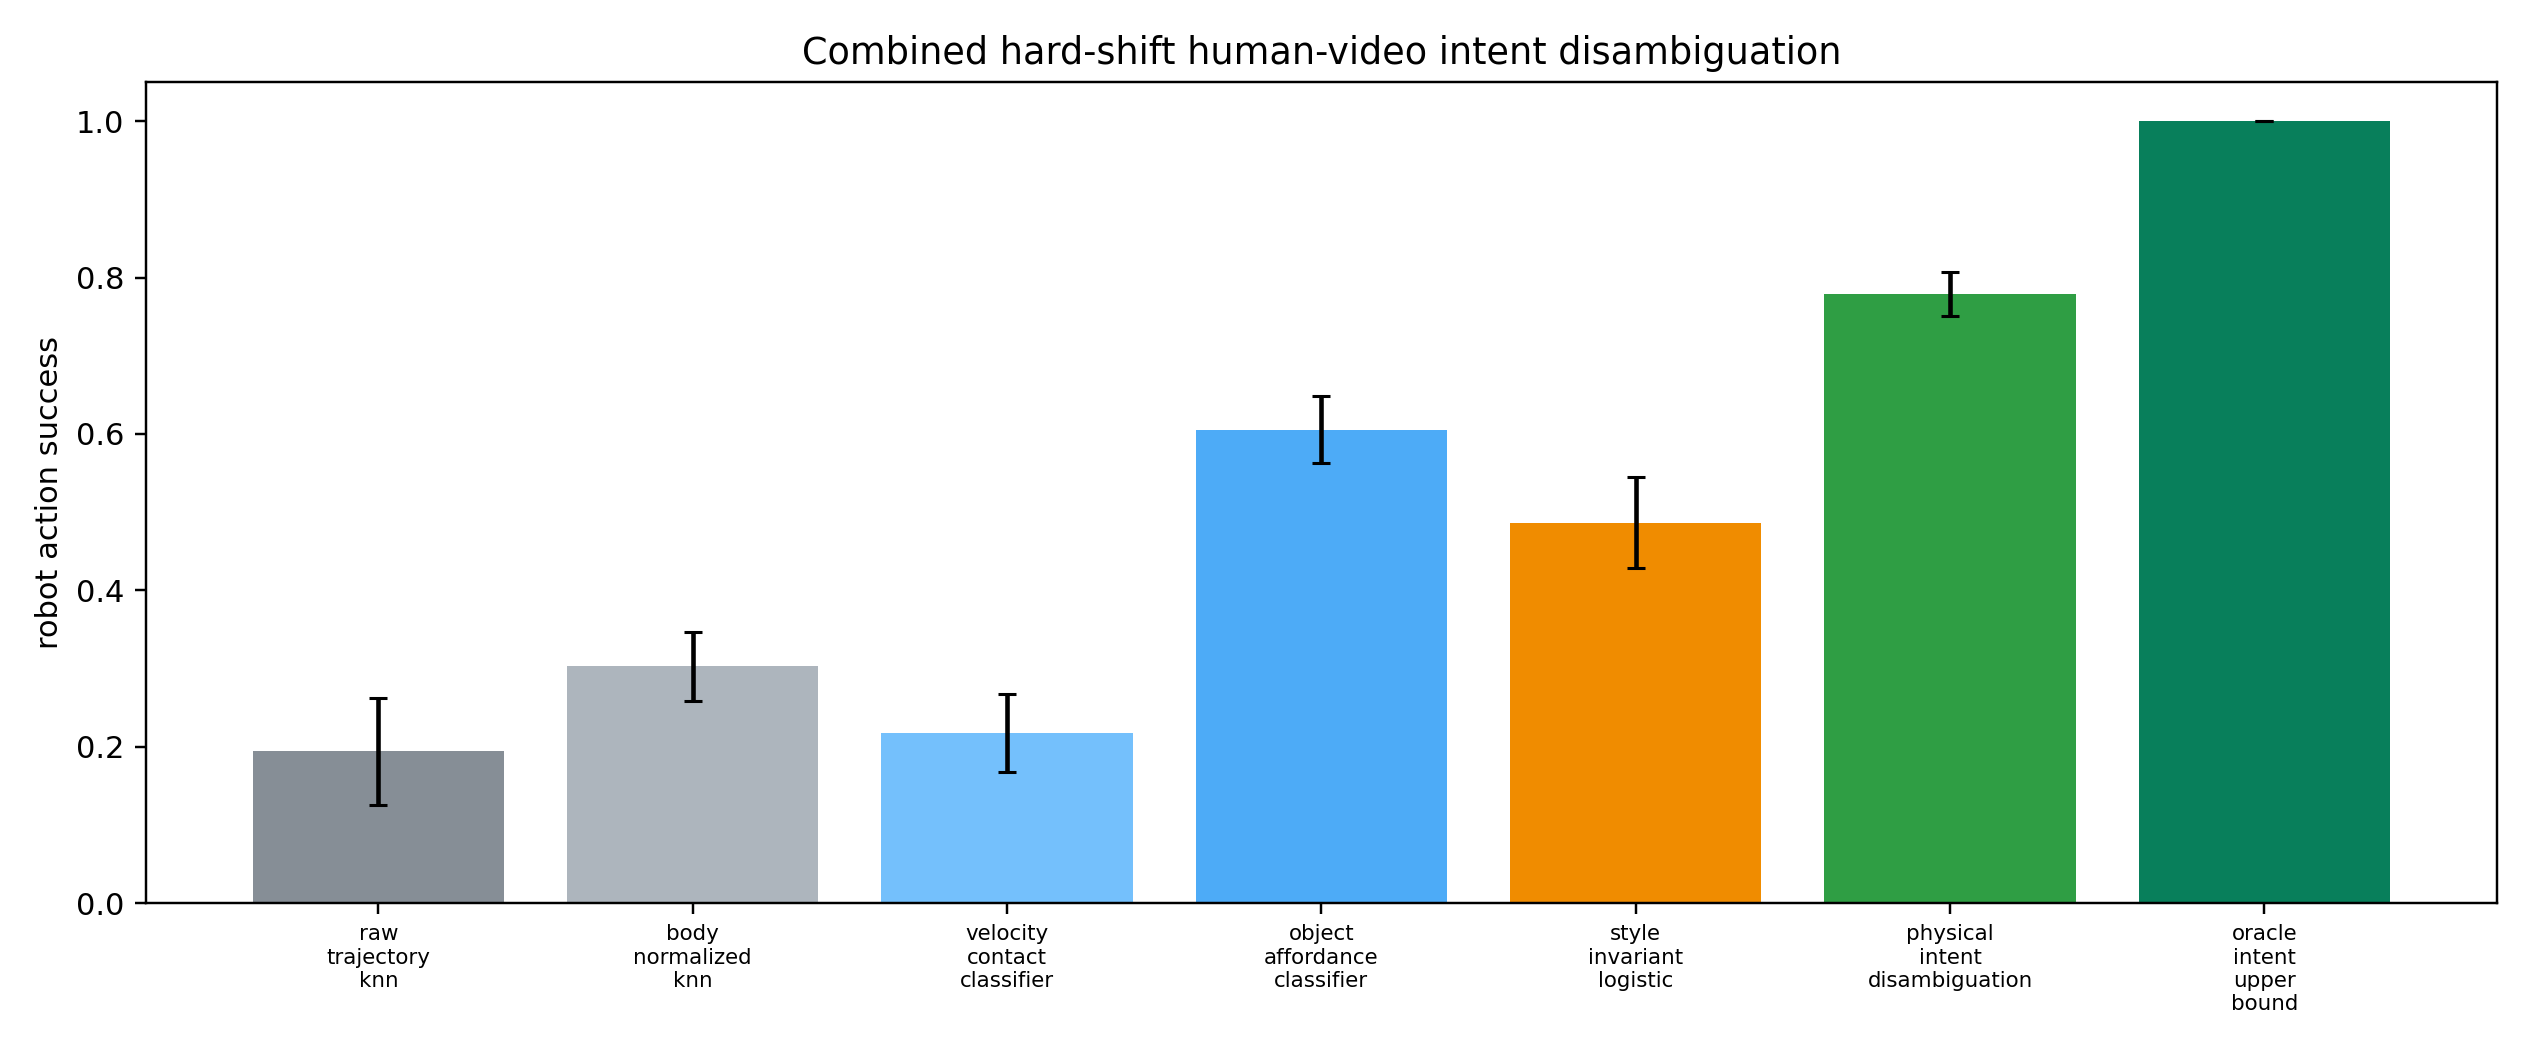
\includegraphics[width=0.95\linewidth]{../figures/intent_success_combined.png}
\caption{Combined hard-shift action success. The factored physical-intent model beats the strongest non-oracle baseline.}
\end{figure}

\section{Morphology Leakage}
We measure morphology leakage by training a probe to recover body-scale group from the representation. Raw video features leak morphology strongly at $0.782$ probe accuracy. The proposed factored representation reduces leakage to $0.578$, while retaining higher robot action success than morphology-blind object-only features.

\begin{figure}[tbp]
\centering
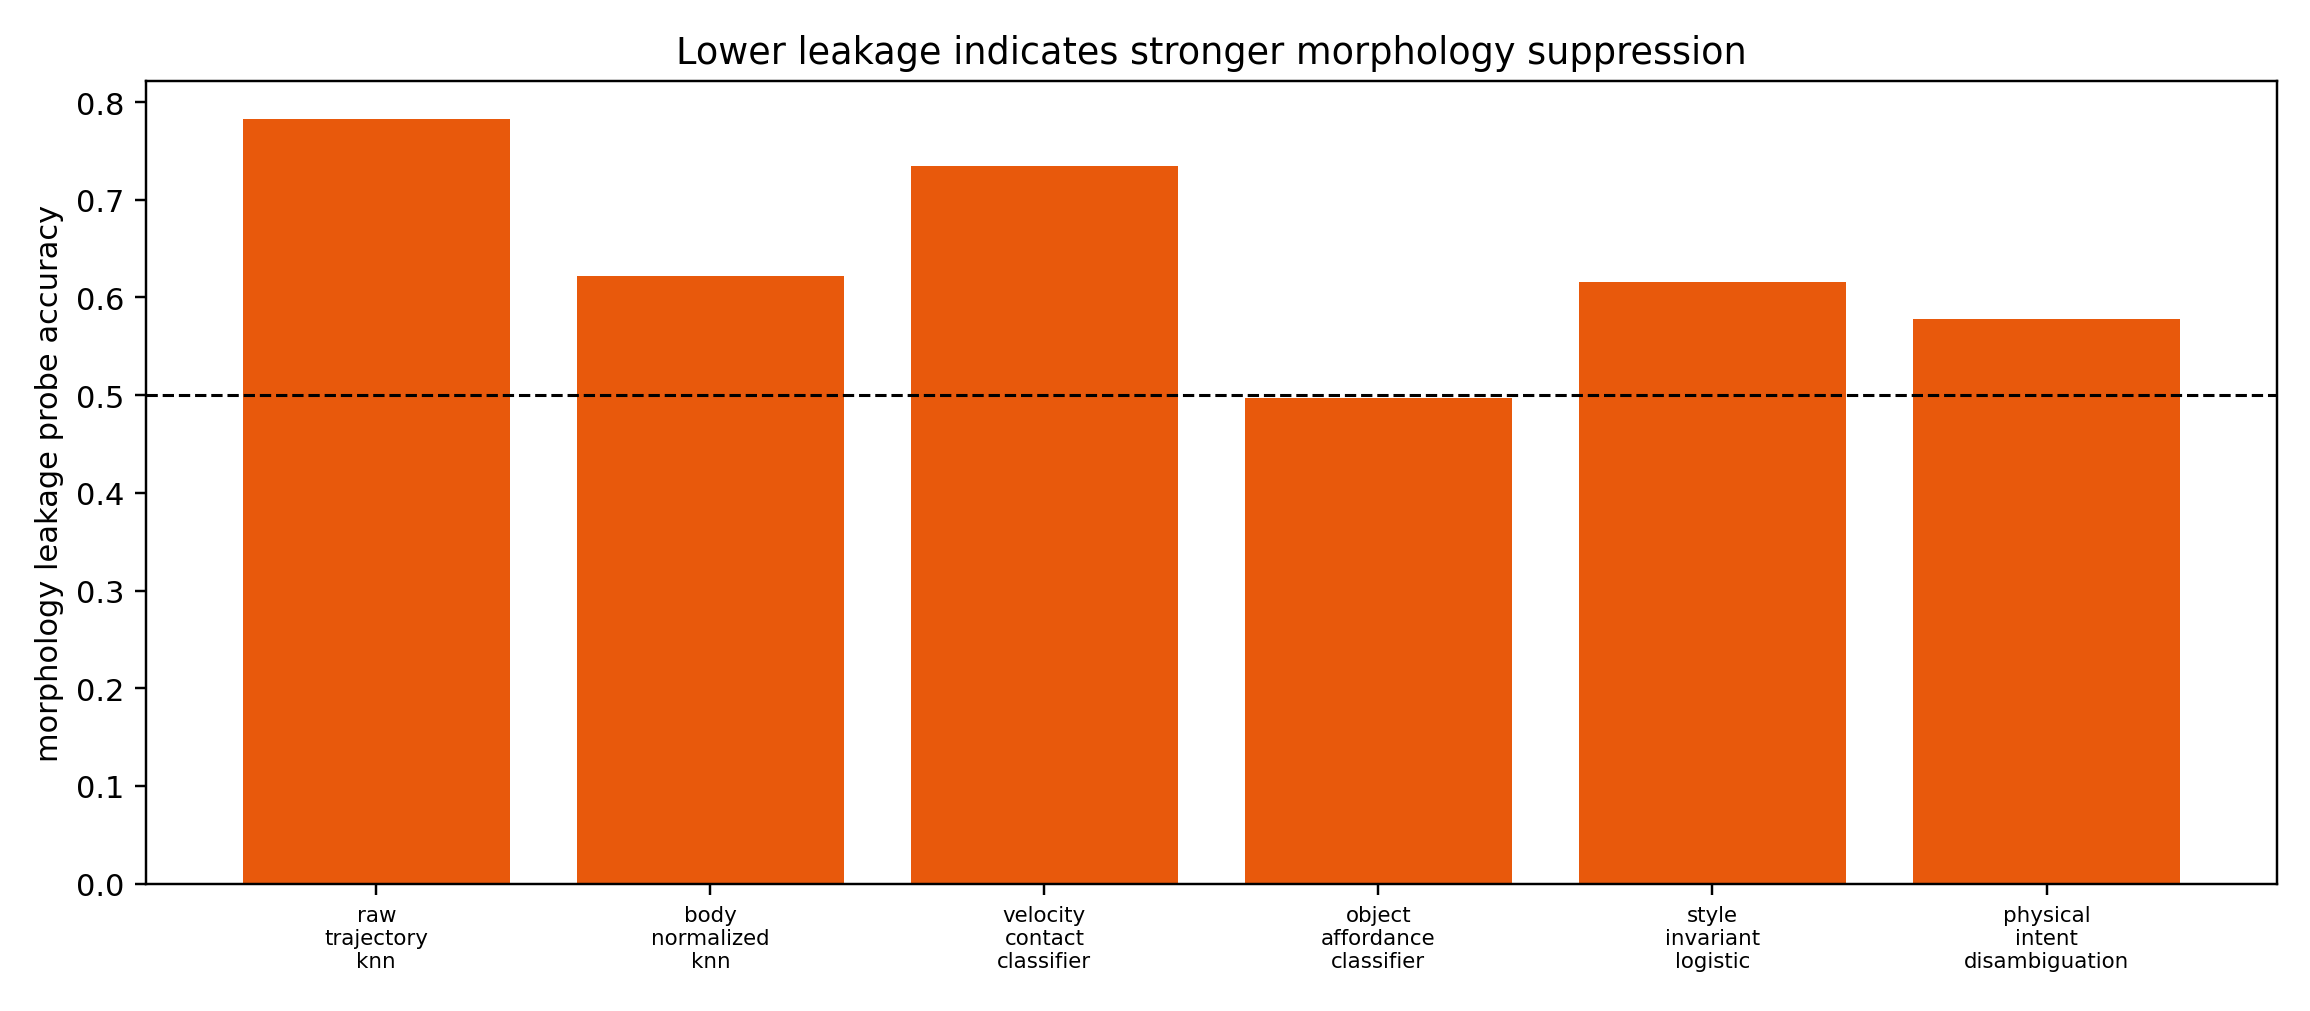
\includegraphics[width=0.95\linewidth]{../figures/morphology_leakage.png}
\caption{Morphology leakage probe accuracy on \texttt{combined\_hard\_shift}. Lower is better; dashed line indicates chance.}
\end{figure}

\section{Ablations}
Table~\ref{tab:ablations} shows ablations on \texttt{combined\_hard\_shift}. Removing object-affordance evidence causes the largest drop, from $0.779$ to $0.663$ action success. Removing style-speed normalization is smaller but negative. Body-scale and handedness ablations are modest, which weakens any claim that every morphology term is independently necessary. Contact timing and uncertainty gating are nearly neutral in this local benchmark.

\begin{table}[tbp]
\centering
\scriptsize
\setlength{\tabcolsep}{4pt}
\begin{tabular}{lccc}
\toprule
Ablation & Action success & Intent acc. & Param. error \\
\midrule
Full method & $0.779 \pm 0.028$ & $0.796$ & $0.171$ \\
Minus body-scale normalization & $0.769 \pm 0.043$ & $0.789$ & $0.169$ \\
Minus handedness mirroring & $0.765 \pm 0.031$ & $0.786$ & $0.169$ \\
Minus object affordance & $0.663 \pm 0.039$ & $0.667$ & $0.297$ \\
Minus contact timing & $0.779 \pm 0.030$ & $0.806$ & $0.165$ \\
Minus style-speed normalization & $0.755 \pm 0.028$ & $0.776$ & $0.172$ \\
Minus uncertainty gate & $0.782 \pm 0.028$ & $0.796$ & $0.171$ \\
\bottomrule
\end{tabular}
\caption{Ablations. The object-affordance component is essential; contact and uncertainty components are not validated by this benchmark.}
\label{tab:ablations}
\end{table}

\begin{figure}[tbp]
\centering
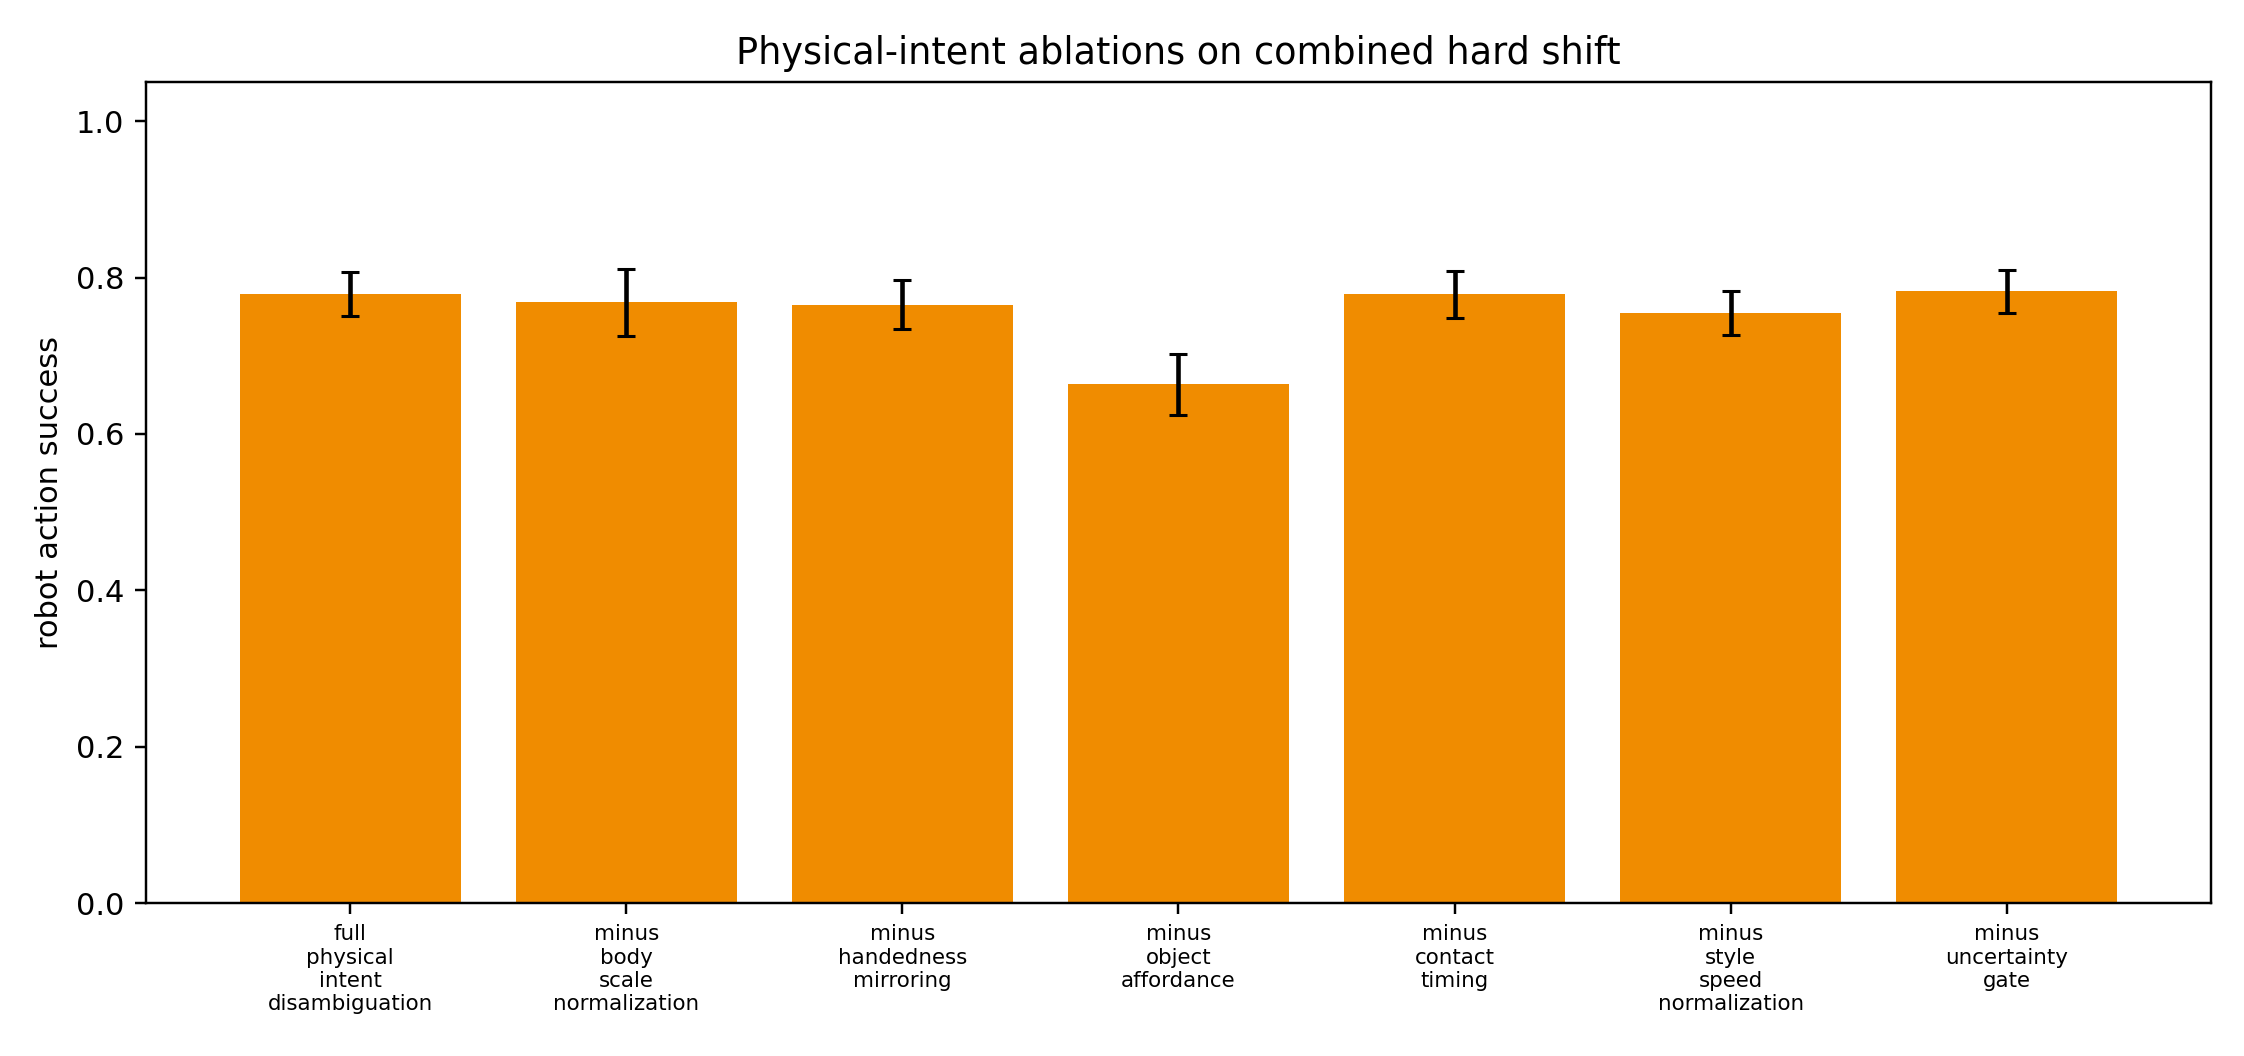
\includegraphics[width=0.95\linewidth]{../figures/intent_ablation.png}
\caption{Ablations on the combined hard split. Neutral ablations are reported rather than hidden.}
\end{figure}

\section{Stress Tests}
Stress sweeps independently vary morphology gap, style exaggeration, affordance ambiguity, and their combination. At maximum combined stress, the proposed method reaches $0.714 \pm 0.045$ action success, compared with $0.518 \pm 0.081$ for object-affordance classification and $0.476 \pm 0.059$ for style-invariant logistic regression.

\begin{figure}[tbp]
\centering
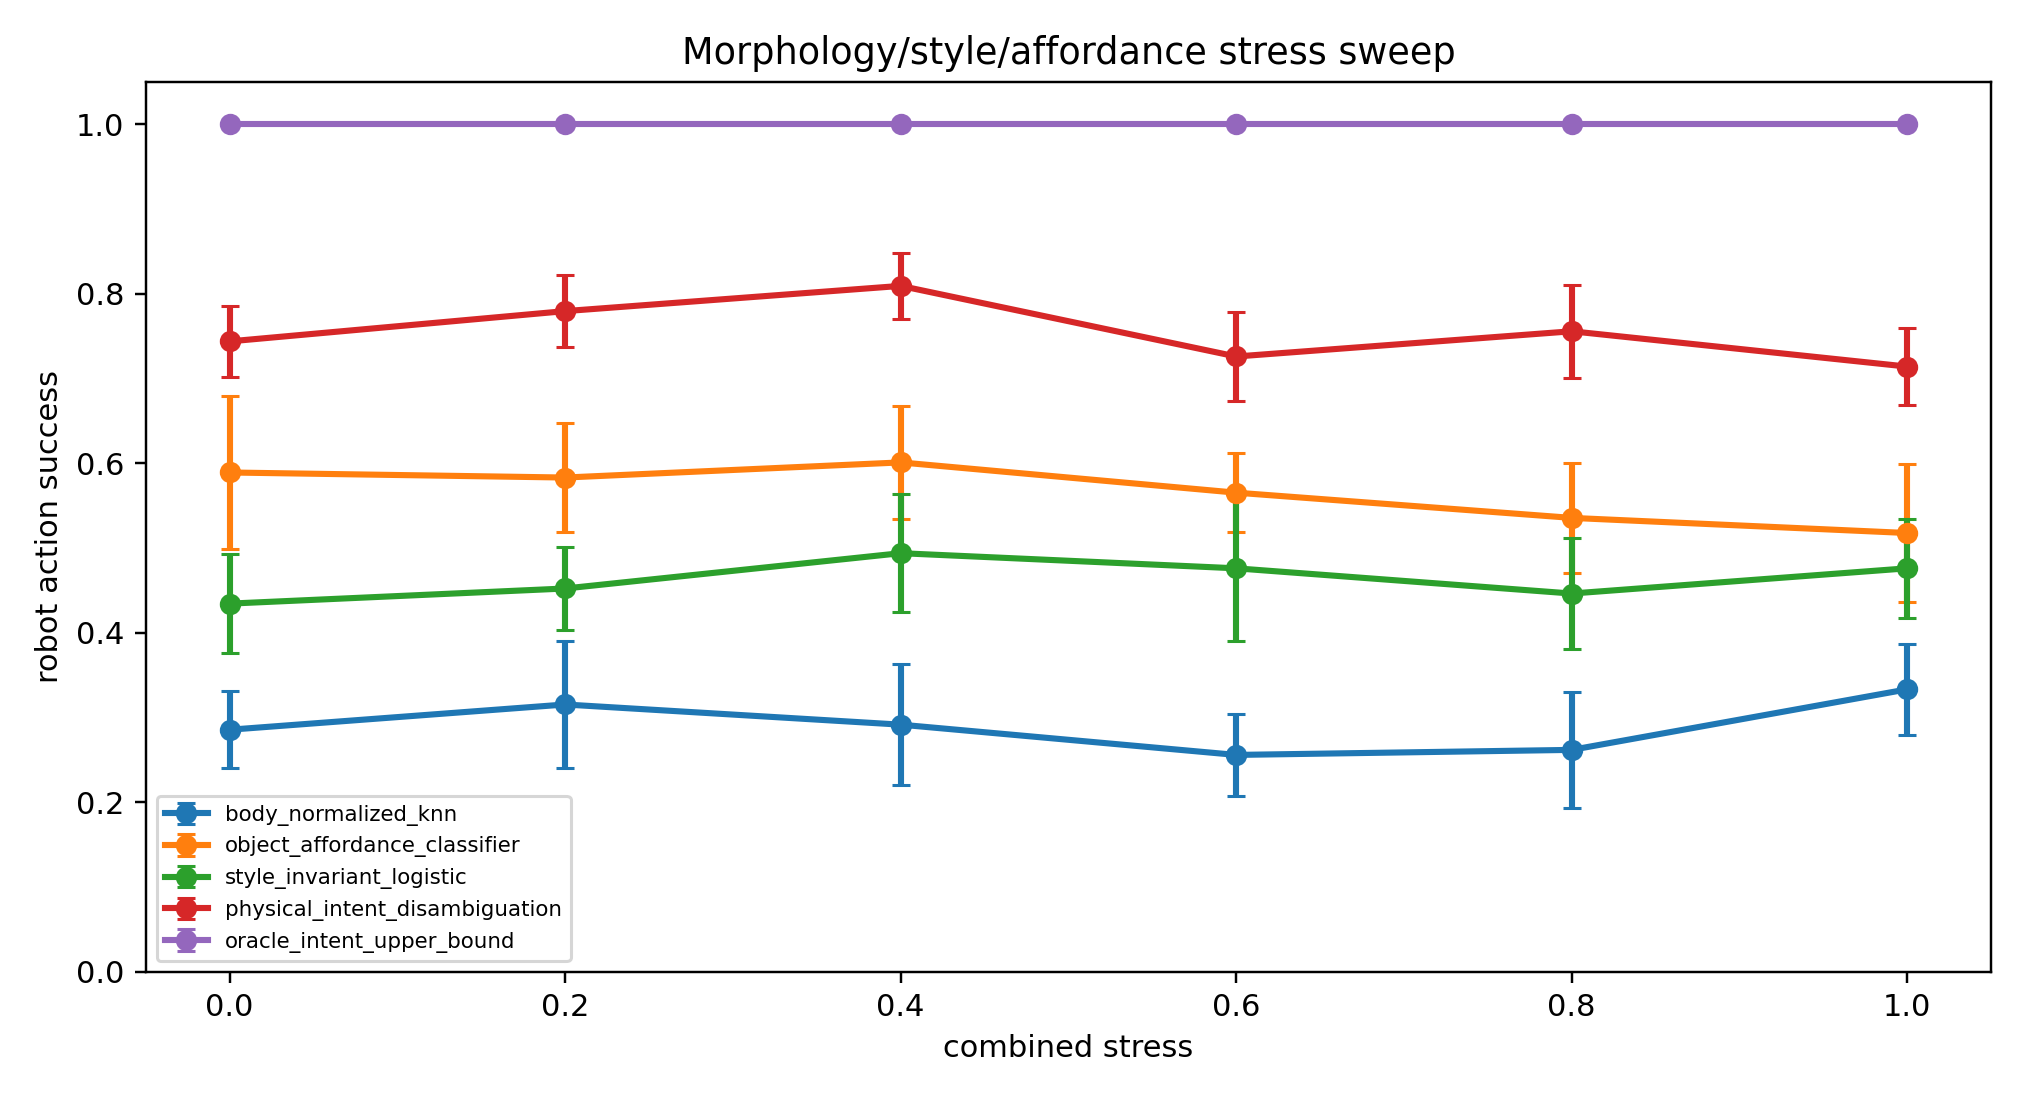
\includegraphics[width=0.95\linewidth]{../figures/intent_stress_sweep.png}
\caption{Combined morphology/style/affordance stress sweep.}
\end{figure}

\section{Related Work Pressure}
The result sits inside crowded literatures on human motion estimation, human intent modeling, robot learning from human video, mirrored demonstrations, and intent-aware physical human-robot interaction \citep{prior1,prior2,prior3,prior4,prior5,prior6,prior8}. A publishable main-conference version must compare against real video-to-robot systems and recognized manipulation benchmarks, not only this local generated benchmark.

\section{Limitations}
This rebuild does not use real human-video datasets, real robot rollouts, external simulators, or learned visual encoders. The benchmark is useful because it makes morphology, style, contact, and affordance confounds explicit, but it is still generated. The neutral contact-timing and uncertainty-gate ablations also narrow the supported claim. The honest next step is to validate the factored representation on real demonstrations or a recognized simulator suite before submission.

\section{Conclusion}
The v4 rebuild changes Paper 80 from an archive-only template into a promising empirical artifact. The proposed factored physical-intent disambiguator beats strong local baselines under combined morphology, style, affordance, occlusion, and noise shifts. The correct terminal state is \textbf{STRONG REVISE}: continue the project, but do not submit to ICLR main until real-video or robot evidence is added.

\bibliographystyle{iclr2026_conference}
\bibliography{references}

\end{document}
